\documentclass{article}

            \usepackage{tikz}
            \usetikzlibrary{calc}
            \title{Young Tableaux}
            \begin{document}
            \maketitle
            \begin{figure}[h]
               \tikzset{
                  tick/.style = {black, very thick}
                }
            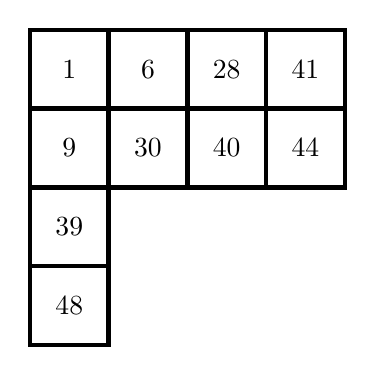
\begin{tikzpicture} % boxlength=1 
            \
\draw [ultra thick] (0,0) rectangle (1,1);
                     \node at ($(0,0)+(0.5,0.5)$) {$48$};
\draw [ultra thick] (0,1) rectangle (1,2);
                     \node at ($(0,1)+(0.5,0.5)$) {$39$};
\draw [ultra thick] (0,2) rectangle (1,3);
                     \node at ($(0,2)+(0.5,0.5)$) {$9$};
\draw [ultra thick] (1,2) rectangle (2,3);
                     \node at ($(1,2)+(0.5,0.5)$) {$30$};
\draw [ultra thick] (2,2) rectangle (3,3);
                     \node at ($(2,2)+(0.5,0.5)$) {$40$};
\draw [ultra thick] (3,2) rectangle (4,3);
                     \node at ($(3,2)+(0.5,0.5)$) {$44$};
\draw [ultra thick] (0,3) rectangle (1,4);
                     \node at ($(0,3)+(0.5,0.5)$) {$1$};
\draw [ultra thick] (1,3) rectangle (2,4);
                     \node at ($(1,3)+(0.5,0.5)$) {$6$};
\draw [ultra thick] (2,3) rectangle (3,4);
                     \node at ($(2,3)+(0.5,0.5)$) {$28$};
\draw [ultra thick] (3,3) rectangle (4,4);
                     \node at ($(3,3)+(0.5,0.5)$) {$41$}; % draw rectangles and numbers, string created by def rectangle_nodes
            \%
            \end{tikzpicture}
            \end{figure}
            \end{document}